%%%%%%%%%%%%%%%%%%%%%%%%%%%%%%%%%%%%%%%%%%%%%%%%%%%%%%%%%%%%%%%%%%%%%%%%%%%%%%%%%%%%%%%%%
% SECTION HYDRODYNAMIC SIMULATIONS 
%%%%%%%%%%%%%%%%%%%%%%%%%%%%%%%%%%%%%%%%%%%%%%%%%%%%%%%%%%%%%%%%%%%%%%%%%%%%%%%%%%%%%%%%%

\chapter{Hydrodynamic Simulations}
\section{Code Description}

The code we used is called SLH (Seven League Hydro). It was originally developed by Dr. Fabian Miczek during his PhD thesis (2013). SLH is a finite-volume multidimensional code that solves Euler equations (Ideal Hydrodynamic) using explicit or implicit methods. The advantage of implicit methods lies in the fact that the time step is constantly redefined optimizing computational resources using the so called cfl criterion for numerical stability. In this case a non-linear system of equations is solved using the Newton-Ralphson method, in which at every time step a linear system is solved through the Krylov subspace methods. The efficiency of all these computational methods is strongly dependent on the type of linear system solved and the cluster architecture used. \\
From the point of view of simulation domain SLH allows to implement a general curvilinear grid instead of a simple cartesian one by defining a metric, the elements of which are needed to correctly compute the fluxes at the cells interfaces. The code decomposes automatically the domain to parallelize the computation on the desired number of processors, using MPI and openMP. A wide choice of boundary conditions are implemented. \\
Furthermore SLH implements a general equation of state, a nuclear reaction network, passive and active scalar which are fundamental for the study of the chemical composition of the fluid, radiation in the diffusion limit and thermal conduction. \\
Over the years SHL has undergone several scaling tests, the most remarkable of which at the Jülich Supercomputing Center (JSC) in 2016 where it scaled over all the $458752$ cores of \textit{JUQUEEN} (a Blue Gene machine, currently the last generation of IBM supercomputers).
\section{2D Simulations}
\subsection{Simulations setup}
The physical setup used for our simulations is the so called "box in a star" method, meaning that we simulate some very small internal region of a star. \\
In our case for the 2D runs it will be a box of $2.50 \times 10^{9} cm$ on the $x$ axis and $1.25 \times 10^{9} cm$ on the $y$ axis. Gravity is constant pointing downward on the $y$ axis with a magnitude of $1000 cm/s^2$. This generates a pressure stratification in the fluid that covers approximately three pressure scale heights. \\
The controlling parameter in our setup is the temperature gradient that can be initialized to any value. In our case we divided the simulated region in three parts. The bottom region (labeled as $1$) starts at the lower boundary and reaches $4/12$ of the domain, the central (labeled as $2$) proceeds till the middle, and the upper one (labeled as $3$) reaches the upper boundary, as shown in \ref{fig:tempprofile}. We define a parameter $\alpha_{i}$ ($i=1, 2, 3$) which is nothing but the fraction of the $\nabla$ over the $\nabla_{\mathrm{ad}}$. As seen in previous sections $\alpha_{i}<1$ implies stability in the $i-$region, instability otherwise. \\
We always initialized the setup with $\alpha_{1} = \alpha_{3}$ widely smaller than $1$; and $\alpha_{2}=0.99$, which means a very precarious situation in terms of stability in the second region. A heating function furthermore heats the second region with a gaussian profile (see \label{fig:tempprofile}) to generate convection that will expand downward and upward by entrainment. The values of $\alpha_{1}$ and $\alpha_{3}$ are controlling parameters for the bulk-Richardson number, since they are proportional to $\Delta b$. The advantage of simulating a strip of convection between two stable layers (miming a Shell convection) instead of a convective region at the bottom that grows upward (Core convection-like) is twofold: it gives us two convective boundaries to study instead of one, and we avoid high mach number at the boundary which can at times generate problems or unphysical situations. \\
One of the hardest tasks has been to generate the correct amount of heating such that the turbulence standard deviation \textit{at the interface} was constant during the run (which is one of the ingredients of the bulk-Richardson number, hence one of the parameters we want to control in order to perform a differential study). In order to do that, the heating function is tuned such that, at $t=100K s$ the total heat generation is reduced to $50 \%$ of the original amount.\\ 
\begin{figure}[t]
\centering
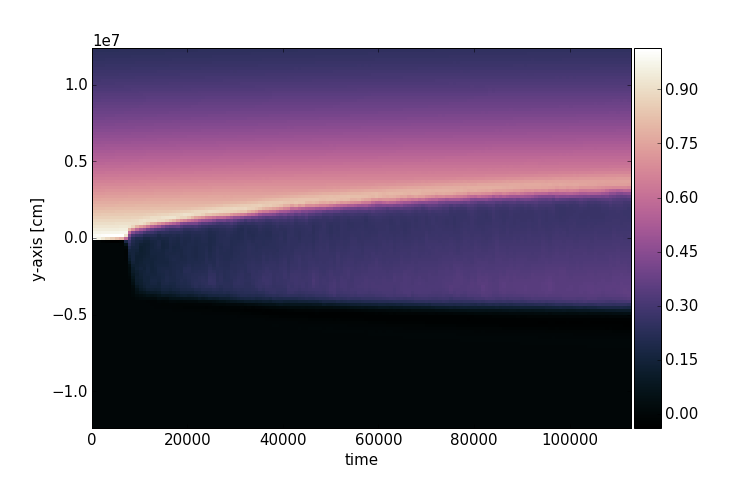
\includegraphics[width=10cm]{./img/tempprofile}
\caption{Example of initial temperature profile along the $y$-axis}
\label{fig:tempprofile}
\centering
\end{figure}
At the bottom of the simulated region small perturbations in temperature and mach number had been imprinted on the stratification in order to break the initial symmetry of the system.\\
A wide range of boundary conditions have been tested for this problem. We used for the horizontal direction periodic boundaries, that definitely provide the most physical situation. For the vertical direction we used wall boundary conditions.\\ 
As briefly explained in the previous sections, in order to define the topology of the convective boundaries, we initialized a passive scalar inside each one of the regions. Recall that passive scalars are just like colors of the fluid and in no way they influence the dynamic of the system, neither they diffuse.\\
As previously stated our goal is to perform a \textit{differential} study of the bulk-Richardson number and the CBM problem. This implies running simulations with different values of $\Delta b$ and $\sigma_t$ at different resolutions. Being 2D simulations computationally so cheap, we managed to run a copious amount of them. With the code 2d0.10-0.80 we will refer to a 2-dimensonal run with $\alpha_{1} = \alpha_{3}=0.1$ and $80 \%$ of the heating referring to the arbitrary value of $4.5 10^{15} \mathrm{erg/s}$.\\ 
We run in 2D on a $2048 \times 1024$ uniform Cartesian grid. It is worth remarking that when doing CFD with a higher resolution, one not only resolves better the features of the system, but also decreases the numerical viscosity (increases the Reynolds number). This is the reason for which we chose this grid setup: we want to keep cells squared and keep viscosity a scalar quantity, and prevent it from becoming a tensorial one. In the next section we will perform a convergence study, in order to undertand which roles the resolution and the viscosity play in the phenomenon of convective entrainment.\\ 

\subsection{Evolution of a single run}



\begin{figure}[t]
      \centering
        \subfloat[Mach number profile over time.]{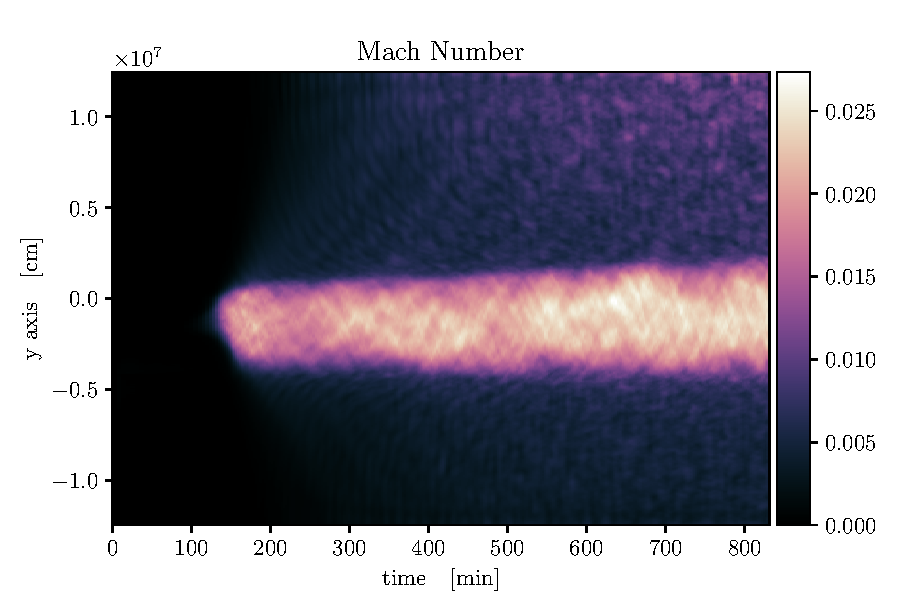
\includegraphics[width=10cm]{./img/mach.pdf}\label{fig:2d0.7-0.01LR.turbmach}}
     \centering
	\hfill
        \subfloat[Entrainment of passive scalar from the upper stable region in the convective region.]{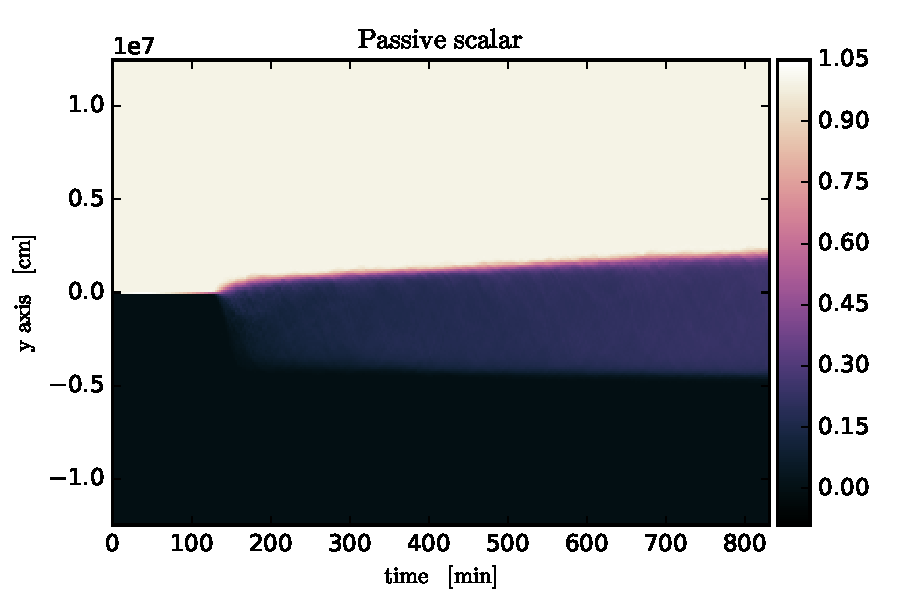
\includegraphics[width=10cm]{./img/ps2.pdf}\label{fig:2d0.7-0.01LR.bp}}
\end{figure}
 %%%%%%%
 % divisione figure %
 %%%%%%%
\begin{figure}[t]
  \centering
    \subfloat[Bulk-Richardson number over time.]{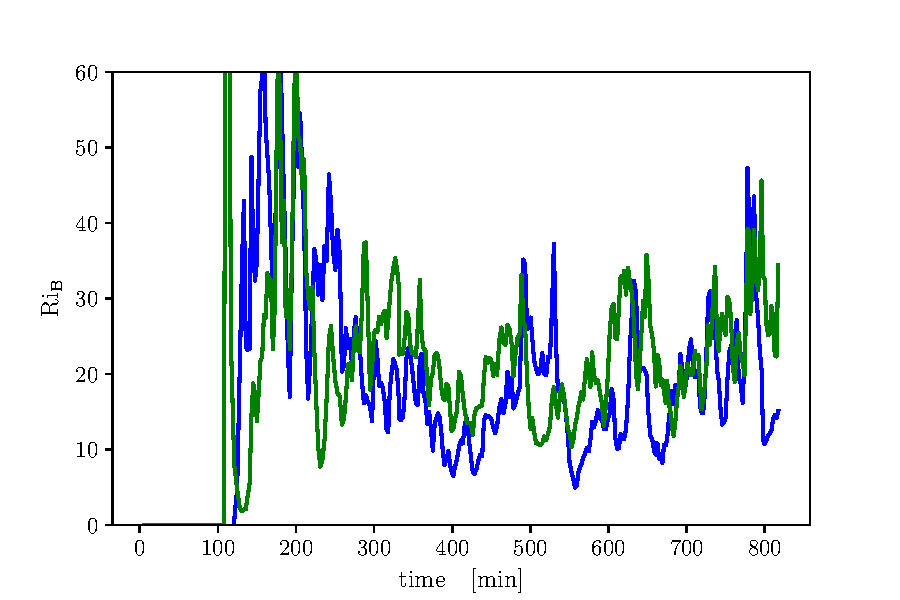
\includegraphics[width=0.5\textwidth]{./img/bulk.pdf}\label{fig:bulk}}
      \hfill
        \subfloat[Entrained mass over time.]{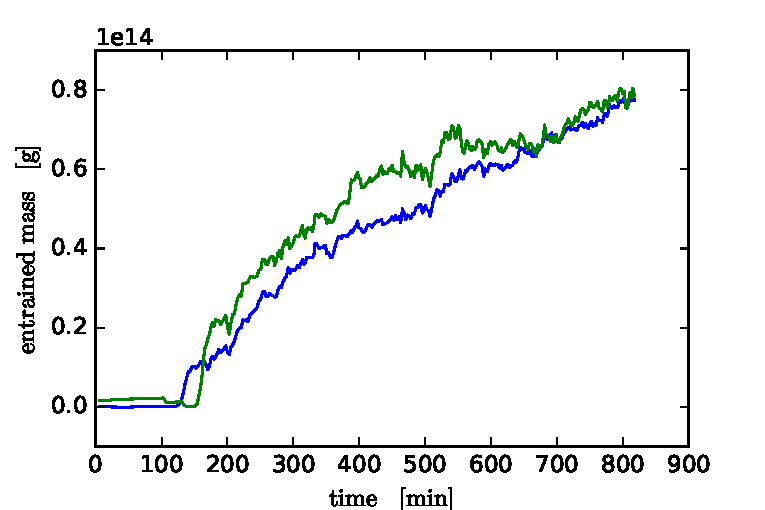
\includegraphics[width=0.5\textwidth]{./img/ent.pdf}\label{fig:2d0.7-0.01LR.ent}}
	\hfill
  \centering
    \subfloat[Turbulence standard deviation over time.]{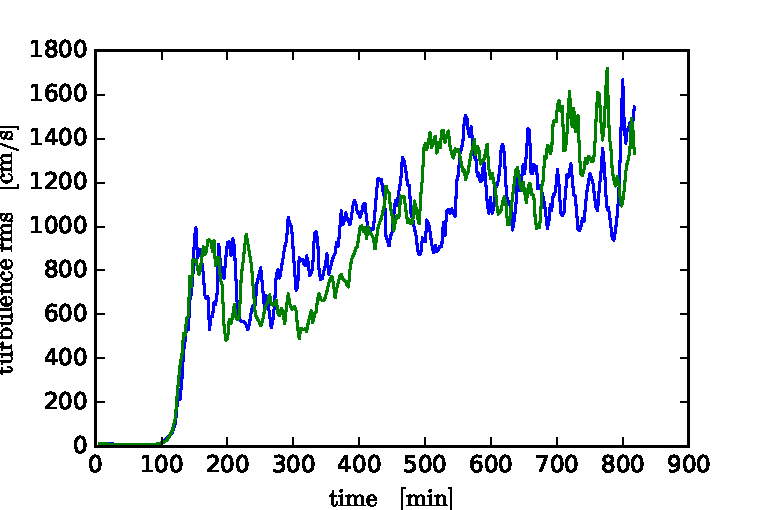
\includegraphics[width=0.5\textwidth]{./img/sigt.pdf}\label{fig:sigt}}
      \hfill
        \subfloat[Turbulence length scale over time.]{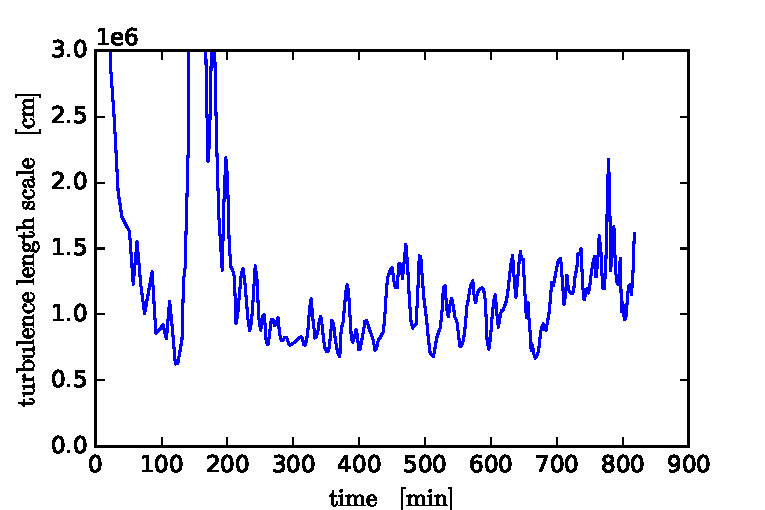
\includegraphics[width=0.5\textwidth]{./img/len.pdf}\label{fig:2d0.7-0.01LR.turbmach}}
	\hfill
  \centering
    \subfloat[Buoyancy jump over time.]{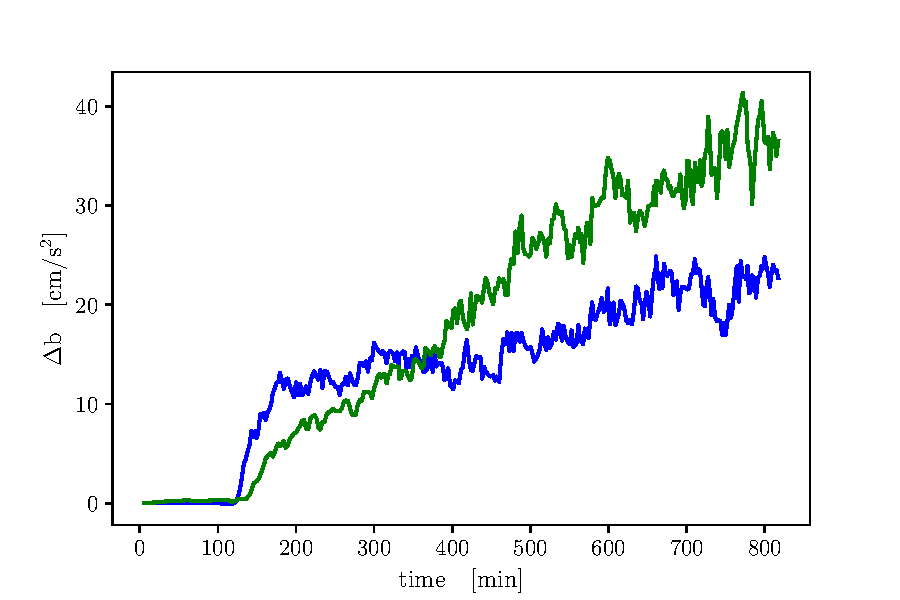
\includegraphics[width=0.5\textwidth]{./img/delb.pdf}\label{fig:2d0.7-0.01LR.bp}}
      \hfill
        \subfloat[Bounday position and width over time.]{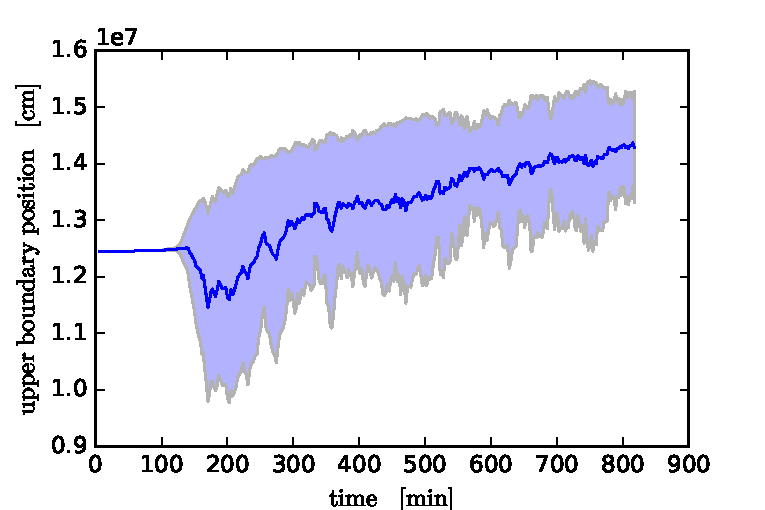
\includegraphics[width=0.5\textwidth]{./img/boundpos.pdf}\label{fig:2d0.7-0.01LR.turbmach}}
	\caption{Plots of the relevant parameters for our analysis over time.}
	  \label{fig:2dsingle}
  \end{figure}

Let's consider the setup 2d0.1-0.80. \\
Convection starts at around $t \sim 7000 s$. Because of the already mentioned implicit time stepping, the lower the mach number, the bigger the time step, allowing us to save a huge amount of computational resources before the rise of convection. A remarkable difference is also observed in the convective regime, as long as the mach number is below $10 \%$, which has always been our case.\\
In figure \ref{fig:2d001-LRmach} we plot the profile of the mach number over the simulated time. this is what one would expect, with two remarks that need to be done. \\
First of all the mach number is stable over time, thanks to the heating function that we implemented, featuring a decrease of heat generation as previously explained. \\
Second of all it is clear that some internal modes are excited by the convective blobs when they hit the stable layers and they propagate through it. They appear more significative in the upper region and to a certain extent it's true, but mainly this is due to the fact that the speed of sound there it's lower. Plotting the absolute velocity the difference is not so dramatic. Two intresting questions that remain without answer. First of all it is impossible to tell to which extent the dynamic of the boundary is influenced by these modes. Second of all it is possible that the chemical mixing due to these modes in the stable stratification might have a significant impact on the evolution of a star, which is obviously not considered in 1-D simulations.\\
In figure \ref{fig:2dsingle} we plot the passive scalar initialized inside the upper region, which over time is entrained by convection. We clearly see the movement of the boundaries that over the $60000 s$ of simulated time move gradually upward and downward. Specifically in the upper case it starts in the middle of the simulated region and ends up at $\sim 8.0 \times 10^{6} cm$, for the lower case it starts at $\sim 3.7 \times 10^{6} cm$ and moves downwards toin the middle of the simulated region \\
In figure \ref{fig:2dsingle} we plot some parameters relevant to our analysis. \\
We show first of all the bulk-Richardson number over time. At around $t=\mathrm{300 \ min}$, when the entrainment becomes linear, the bulk-Richardson number still oscillates over half an order of magnitude. This obviously deeply affects our data analysis, making necessary a large amount of runs to collect as more data as possible. This also makes impracticable a differential study of the entrainment over time. \\
Second of all we plot in figure \ref{fig:ent} the entrained mass over time. As already mentioned we will perform a lagrangian study of entrainment, because it is impracticable to quantify how much of the boundary movement is due to the entrained mass or to the adiabatic expansion of the fluid. We notice that also the entrainment rate stabilizes after the initial transition. \\
  In figure \ref{fig:sigt} we plot the turbulence standard deviation over time. It is overall constant, with a slight trend to increase. This result has been obtained after extensive tests to correctly tune the heating function.\\
At last we plot in figure \ref{fig:2d0.7-0.01LR.l} the bulk-Richardson number over time.\\
For every 2D or 3D run we will extrapolate the relevant parameters and present them in the following layout
\begin{center}
 \begin{tabular}{l|c|c|c|c|c}
	 Run & $\Delta b$  $(\mathrm{cm/s^{2}})$ & $\sigma_t$ $(\mathrm{cm/s})$ & $L$ $(\mathrm{cm})$ & $Ri_{\mathrm{B}}$ & $\dot{M}_{\mathrm{exp}}$ $(\mathrm{g/s})$\\
	  	\hline
		2d0.7-0.01U & 21.84 & 1174 & $1.7 \times 10^{7}$ & 290.57  & $1.2 \times 10^{9}$ \\
		\hline
		2d0.7-0.01L & 43.73 & 1179 & $1.7 \times 10^{7}$ & 567.68 & $8.1 \times 10^{8}$ \\ 
      \end{tabular}
 \end{center}

\subsection{Resolution study}
\begin{figure}[b!]
  \centering
    \subfloat[Mach number profile for the $2048 \times 1024$ run.]{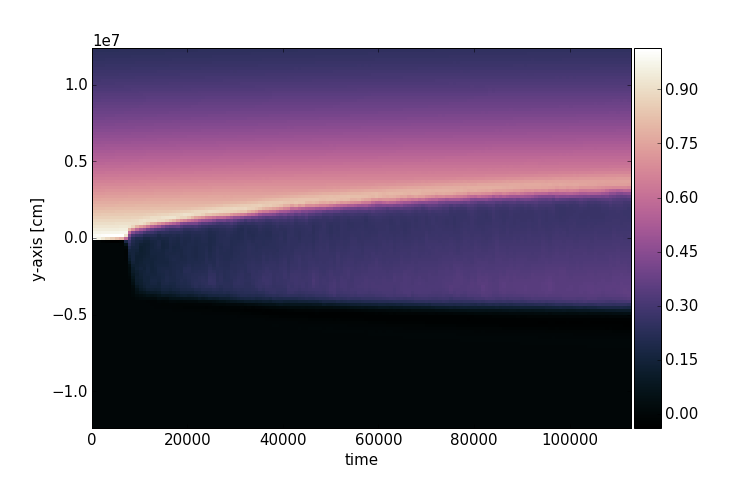
\includegraphics[width=0.5\textwidth]{./img/tempprofile}}
      \hfill
  \centering
    \subfloat[Mach number profile for the $512 \times 256$ run.]{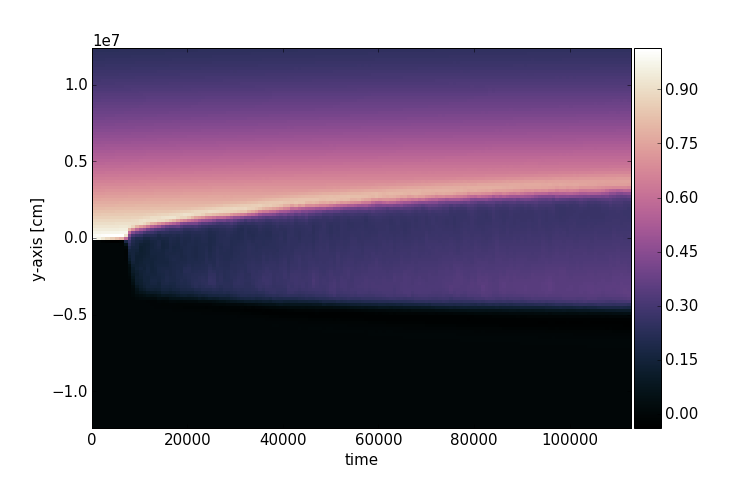
\includegraphics[width=0.5\textwidth]{./img/tempprofile}}
      \hfill
	\caption{Turbulent structures at different resolutions}
    \label{fig:differentialmach}
  \end{figure}
In the last section we analyzed the run 2d0.10-0.80. What we will do in this section is to compare the previous results with the ones obtained by running the same setup on smaller resolutions, in order to understand if we are properly resolving the system. \\
The same setup was run on a $1024 \times 512$ and $512 \times 256$. As espected, the highest resolution run shows smaller and more refined turbulent structures in the convective region, while in the smallest run we observe less eddies but of bigger size (see figure \ref{fig:differentialmach}).\\
As previously found by Woodward \textit{et al.} 2016 \cite{woodward} the enhanced the resolution, the lower the entrainment rate, with 

\section{Differential study}
